\documentclass{beamer}

	\title{Path Planning for Cable Driven Parallel Robots\\Literature Study}
	\author{Hendrik Scheepers de Bruin}
	\institute{École Centrale de Nantes, Università degli Studi di Genova}
	\date{January 2019}

    \usepackage{graphicx}
		\graphicspath{{res/img/}}
	\usepackage{import}

    \usepackage{mathrsfs}
    \usepackage{amsfonts}
    \usepackage{amssymb}
    \usepackage{dsfont}
	\usepackage{amsmath}
    \usepackage{mathtools}
    \usepackage{ifdraft}
    \usepackage[section=subsection, acronyms]{glossaries}
        \makenoidxglossaries{}
        % Dependencies:
%	*	mathrsfs	- for mathscr font
%	*	amsfonts	- for mathfrak and mathbb (upper case) letters
%	*	amssym		- for backepsilon
%	*	dsfont		- for mathds
\newglossary*{notation}{Notation}

% ==============================================================================
% Scalar
% ==============================================================================
	\newglossaryentry{not:scalar}
	{%
		name=\ensuremath{m},
		description=a scalar,
		type=notation
	}
	\glsadd{not:scalar}

% ==============================================================================
% Vector
% ==============================================================================
	\renewcommand{\vec}[1]{\ensuremath{\boldsymbol{#1}}}
	\newglossaryentry{not:vec}
	{%
		name=\vec{m}\ifdraft{: \textbackslash{} vec}{},
		description=a vector,
		type=notation
	}
	\glsadd{not:vec}

% ==============================================================================
% Projection
% ==============================================================================
	\newcommand{\project}[2]{\ensuremath{{}^{#2}\!{#1}}}
	\newglossaryentry{not:project}
	{%
		name=\project{\vec{m}}{n}\ifdraft{: \textbackslash{} project\{to\}}{},,
		description=projection of vector \vec{m} in frame $n$,
		type=notation
	}
	\glsadd{not:project}

% ==============================================================================
% Skew Matrix
% ==============================================================================
	\newcommand{\skewmat}[1]{\ensuremath{\widehat{#1}}}
	%\newcommand{\skewmat}[1]{\ensuremath{\left[{#1}\right]_{\mathrm{X}}}}
	\newglossaryentry{not:skewmat}
	{%
		name=\skewmat{\vec{m}}\ifdraft{: \textbackslash{} skew}{},
		description=the skew matrix associated with the vector \vec{m},
		type=notation
	}
	\glsadd{not:skewmat}

% ==============================================================================
% Matrix
% ==============================================================================
	\newcommand{\mat}[1]{\ensuremath{\boldsymbol{\mathrm{#1}}}}
	\newglossaryentry{not:mat}
	{%
		name=\mat{M}\ifdraft{: \textbackslash{} mat}{},
		description=a matrix,
		type=notation
	}
	\glsadd{not:mat}

% ==============================================================================
% Pseudo Inverse
% ==============================================================================
	\newcommand{\pseudoinv}[1]{\ensuremath{{#1}^{+}}}
	\newglossaryentry{not:pseudoinv}
	{%
		name=\pseudoinv{\mat{M}}\ifdraft{: \textbackslash{} pseudoinv}{},
		description=the pseudo inverse of matrix \mat{M},
		type=notation
	}
	\glsadd{not:pseudoinv}

% ==============================================================================
% Vector Space
% ==============================================================================
	\newcommand{\vecspace}[1]{\ensuremath{\mathscr{#1}}}
	\newglossaryentry{not:vecspace}
	{%
		name=\vecspace{M}\ifdraft{: \textbackslash{} vecspace}{},
		description=a vector space,
		type=notation
	}
	\glsadd{not:vecspace}

% ==============================================================================
% Set
% ==============================================================================
	\newcommand{\set}[1]{\ensuremath{\mathcal{#1}}}
	\newglossaryentry{not:set}
	{%
		name=\set{M}\ifdraft{: \textbackslash{} set}{},
		description=a set,
		type=notation
	}
	\glsadd{not:set}

% ==============================================================================
% Function
% ==============================================================================
	\newcommand{\func}[1]{\ensuremath{\mathrm{#1}}}
	\newglossaryentry{not:func}
	{%
		name=\func{m}\ifdraft{: \textbackslash{} func}{},
		description=a function,
		type=notation
	}
	\glsadd{not:func}

% ==============================================================================
% Vector Function
% ==============================================================================
	\newcommand{\vecfunc}[1]{\ensuremath{\boldsymbol{\mathrm{#1}}}}
	\newglossaryentry{not:vecfunc}
	{%
		name=\vecfunc{m}\ifdraft{: \textbackslash{} vecfunc}{},
		description=a vector function,
		type=notation
	}
	\glsadd{not:vecfunc}

% ==============================================================================
% Estimate
% ==============================================================================
	\newcommand{\estimate}[1]{\ensuremath{\widetilde{#1}}}
	\newglossaryentry{not:estimate}
	{%
		name=\estimate{m}\ifdraft{: \textbackslash{} estimate}{},
		description=an estimate of the quantity $m$,
		type=notation
	}
	\glsadd{not:estimate}

% ==============================================================================
% nth Time Derivative
% ==============================================================================
	\newcommand{\tdern}[2]{\ensuremath{{#1}^{(#2)}}}
	\newglossaryentry{not:tdern}
	{%
		name=\tdern{m}{n}\ifdraft{: \textbackslash{} tdern}{},
		description=the nth time derivative of quantity $m$,
		type=notation
	}
	\glsadd{not:tdern}

% ==============================================================================
% Desired Value
% ==============================================================================
	\newcommand{\desired}[1]{\ensuremath{{#1}^{*}}}
	\newglossaryentry{not:desired}
	{%
		name=\desired{m}\ifdraft{: \textbackslash{} desired}{},
		description=the desired value of $m$,
		type=notation
	}
	\glsadd{not:desired}

% ==============================================================================
% Such That
% ==============================================================================
	\newglossaryentry{not:suchthat}
	{%
		name={\ensuremath{\backepsilon}},
		description=such that,
		type=notation
	}
	\newcommand{\suchthat}{\gls{not:suchthat}}

        \newglossary*{symbol}{Symbols}
% ==============================================================================
% Sample
% ==============================================================================
	\newglossaryentry{sym:sample}
	{%
		name=\ensuremath{\sigma},
		sort=s,
		description=sample,
		type=symbol
	}
	\newcommand{\sample}{\gls{sym:sample}}

% ==============================================================================
% Distance
% ==============================================================================
	\newglossaryentry{sym:distance}
	{%
		name=\ensuremath{d},
		sort=h,
		description=distance,
		type=symbol
	}
	\newcommand{\distance}{\gls{sym:distance}}

% ==============================================================================
% Quaternion
% ==============================================================================
	\newglossaryentry{sym:quaternion}
	{%
		name=\ensuremath{\vec{h}},
		sort=h,
		description=quaternion,
		type=symbol
	}
	\newcommand{\quaternion}{\gls{sym:quaternion}}

% ==============================================================================
% Queue
% ==============================================================================
	\newglossaryentry{sym:queue}
	{%
		name=\ensuremath{\code{q}},
		sort=q,
		description=queue,
		type=symbol
	}
	\newcommand{\queue}{\gls{sym:queue}}

% ==============================================================================
% Torque
% ==============================================================================
	\newglossaryentry{sym:torque}
	{%
		name=\ensuremath{\vec{\tau}},
		sort=t,
		description=torque,
		type=symbol
	}
	\newcommand{\torque}{\gls{sym:torque}}

% ==============================================================================
% Gain
% ==============================================================================
	\newglossaryentry{sym:gain}
	{%
		name={\ensuremath{\lambda}},
		sort=l,
		description=A tunable gain,
		type=symbol
	}
	\newcommand{\gain}{\gls{sym:gain}}

% ==============================================================================
% Point
% ==============================================================================
	\newglossaryentry{sym:point}
	{%
		name={\ensuremath{\vec{p}}},
		sort=p,
		description=A point in space,
		type=symbol
	}
	\newcommand{\point}{\gls{sym:point}}

% ==============================================================================
% Set of Points
% ==============================================================================
	\newglossaryentry{sym:setofpoints}
	{%
		name={\ensuremath{\set{P}}},
		sort=p,
		description=A set of points in space,
		type=symbol
	}
	\newcommand{\setofpoints}{\gls{sym:setofpoints}}

% ==============================================================================
% Trajectory
% ==============================================================================
	\newglossaryentry{sym:traj}
	{%
		name={\ensuremath{\vec{s}}},
		sort=s,
		description=A trajectory in space,
		type=symbol
	}
	\newcommand{\traj}{\gls{sym:traj}}

% ==============================================================================
% Path
% ==============================================================================
	\newcommand{\pathsym}{\traj}


% ==============================================================================
% Time
% ==============================================================================
	\newglossaryentry{sym:time}
	{%
		name={\ensuremath{t}},
		sort=t,
		description=time,
		type=symbol
	}
	\newcommand{\timesym}{\gls{sym:time}}

% ==============================================================================
% Time Normalised
% ==============================================================================
	\newglossaryentry{sym:timenorm}
	{%
		name={\ensuremath{\tau}},
		sort=t,
		description=normalised time \ensuremath{\tau \in [0, 1]},
		type=symbol
	}
	\newcommand{\timenorm}{\gls{sym:timenorm}}

% ==============================================================================
% Set of Time Instants
% ==============================================================================
	\newglossaryentry{sym:setoftimeinstants}
	{%
		name={\ensuremath{\set{T}}},
		sort=t,
		description=A set of time instants,
		type=symbol
	}
	\newcommand{\setoftimeinstants}{\gls{sym:setoftimeinstants}}

% ==============================================================================
% Period
% ==============================================================================
	\newglossaryentry{sym:period}
	{%
		name={\ensuremath{T}},
		sort=t,
		description=period,
		type=symbol
	}
	\newcommand{\period}{\gls{sym:period}}

% ==============================================================================
% Tolerance
% ==============================================================================
	\newglossaryentry{sym:tolerance}
	{%
		name={\ensuremath{\epsilon}},
		sort=e,
		description=Tolerance,
		type=symbol
	}
	\newcommand{\tol}{\gls{sym:tolerance}}

% ==============================================================================
% Geometric Model
% ==============================================================================
	\newglossaryentry{sym:geometricmodel}
	{%
		name={\ensuremath{\vecfunc{g}}},
		sort=G,
		description=Geometric Model,
		type=symbol
	}
	\newcommand{\geometricmodel}{\gls{sym:geometricmodel}}

% ==============================================================================
% Inverse Geometric Model
% ==============================================================================
	\newglossaryentry{sym:invgeometricmodel}
	{%
		name={\ensuremath{{\vecfunc{g}^{-1}}}},
		sort=G,
		description=Inverse Geometric Model,
		type=symbol
	}
	\newcommand{\invgeometricmodel}{\gls{sym:invgeometricmodel}}
% ==============================================================================
% Kinematic Model
% ==============================================================================
	\newglossaryentry{sym:kinematicmodel}
	{%
		name={\ensuremath{\vecfunc{k}}},
		sort=K,
		description=Kinematic Model,
		type=symbol
	}
	\newcommand{\kinematicmodel}{\gls{sym:kinematicmodel}}

% ==============================================================================
% Inverse Kinematic Model
% ==============================================================================
	\newglossaryentry{sym:invkinematicmodel}
	{%
		name={\ensuremath{{\vecfunc{k}^{-1}}}},
		sort=K,
		description=Inverse Kinematic Model,
		type=symbol
	}
	\newcommand{\invkinematicmodel}{\gls{sym:invkinematicmodel}}
% ==============================================================================
% Dynamic Model
% ==============================================================================
	\newglossaryentry{sym:dynamicmodel}
	{%
		name={\ensuremath{\vecfunc{d}}},
		sort=d,
		description=Dynamic Model,
		type=symbol
	}
	\newcommand{\dynamicmodel}{\gls{sym:dynamicmodel}}

% ==============================================================================
% Inverse Dynamic Model
% ==============================================================================
	\newglossaryentry{sym:invdynamicmodel}
	{%
		name={\ensuremath{{\vecfunc{d}^{-1}}}},
		sort=d,
		description=Inverse Dynamic Model,
		type=symbol
	}
	\newcommand{\invdynamicmodel}{\gls{sym:invdynamicmodel}}

% ==============================================================================
% Constraint
% ==============================================================================
	\newglossaryentry{sym:constraint}
	{%
		%name=\protect\reflectbox{\ensuremath{\mathds{C}}},
		%name=\protect\reflectbox{\ensuremath{\mat{C}}},
		name=\ensuremath{c},
		sort=c,
		description=constraint,
		type=symbol
	}
	\newcommand{\constraint}{\gls{sym:constraint}}

% ==============================================================================
% Set of Constraints
% ==============================================================================
	\newglossaryentry{sym:setofconstraints}
	{%
		%name=\protect\reflectbox{\ensuremath{\set{C}}},
		%name=\protect\reflectbox{\ensuremath{\mat{C}}},
		name=\ensuremath{\set{C}},
		sort=c,
		description=set of constraints,
		type=symbol
	}
	\newcommand{\setofconstraints}{\gls{sym:setofconstraints}}

% ==============================================================================
% Configuration
% ==============================================================================
	\newglossaryentry{sym:configuration}
	{%
		name=\ensuremath{q},
		sort=q,
		description=Configuration,
		type=symbol
	}
	\newcommand{\configuration}{\gls{sym:configuration}}

%TODO indexes
% ==============================================================================
% Index i
% ==============================================================================
	\newglossaryentry{sym:indexi}
	{%
		name=\ensuremath{i},
		sort=i,
		description=an index,
		type=symbol
	}
	\newcommand{\indexi}{\gls{sym:indexi}}
% ==============================================================================
% Index j
% ==============================================================================
	\newglossaryentry{sym:indexj}
	{%
		name=\ensuremath{j},
		sort=j,
		description=an index,
		type=symbol
	}
	\newcommand{\indexj}{\gls{sym:indexj}}

% ==============================================================================
% Index k
% ==============================================================================
	\newglossaryentry{sym:indexk}
	{%
		name=\ensuremath{k},
		sort=k,
		description=an index,
		type=symbol
	}
	\newcommand{\indexk}{\gls{sym:indexk}}

% ==============================================================================
% State
% ==============================================================================
	\newglossaryentry{sym:state}
	{%
		name=\ensuremath{\vec{x}},
		sort=x,
		description=the state  of the robot,
		type=symbol
	}
	\newcommand{\state}{\gls{sym:state}}

% ==============================================================================
% State Space
% ==============================================================================
	\newglossaryentry{sym:statespace}
	{%
		name=\ensuremath{\vecspace{X}},
		sort=x,
		description=the state space of the robot,
		type=symbol
	}
	\newcommand{\statespace}{\gls{sym:statespace}}

% ==============================================================================
% Inverse Action
% ==============================================================================
	\newglossaryentry{sym:invaction}
	{%
		name=\ensuremath{\vec{u}^{-1}},
		sort=u,
		description=the inverse action  of the robot,
		type=symbol
	}
	\newcommand{\invaction}{\gls{sym:invaction}}
% ==============================================================================
% Action
% ==============================================================================
	\newglossaryentry{sym:action}
	{%
		name=\ensuremath{\vec{u}},
		sort=u,
		description=the action  of the robot,
		type=symbol
	}
	\newcommand{\action}{\gls{sym:action}}

% ==============================================================================
% Action Space
% ==============================================================================
	\newglossaryentry{sym:actionspace}
	{%
		name=\ensuremath{\vecspace{U}},
		sort=u,
		description=the action space of the robot,
		type=symbol
	}
	\newcommand{\actionspace}{\gls{sym:actionspace}}

% ==============================================================================
% Inverse Action Space
% ==============================================================================
	\newglossaryentry{sym:invactionspace}
	{%
		name=\ensuremath{\vecspace{U}^{-1}},
		sort=u,
		description=the inverse action space of the robot,
		type=symbol
	}
	\newcommand{\invactionspace}{\gls{sym:invactionspace}}

% ==============================================================================
% Configuration Space
% ==============================================================================
	\newglossaryentry{sym:configurationspace}
	{%
		name=\ensuremath{\vecspace{C}},
		sort=c,
		description=the configuration space of the robot,
		type=symbol
	}
	\newcommand{\configurationspace}{\gls{sym:configurationspace}}
% ==============================================================================
% World Space
% ==============================================================================
	\newglossaryentry{sym:worldspace}
	{%
		name=\ensuremath{\vecspace{W}},
		sort=w,
		description=the world inhabited by the robot,
		type=symbol
	}
	\newcommand{\world}{\gls{sym:worldspace}}

%%TODO Polynomials
% ==============================================================================
% B-Spline
% ==============================================================================
	\newglossaryentry{sym:bspline}
	{%
		name=\ensuremath{\vec{B}},
		sort=b,
		description=B-spline basis function,
		type=symbol
	}
	\newcommand{\bspline}{\gls{sym:bspline}}
% ==============================================================================
% knot
% ==============================================================================
	\newglossaryentry{sym:knot}
	{%
		name=\ensuremath{\vec{k}},
		sort=k,
		description=B-spline knot vector,
		type=symbol
	}
	\newcommand{\knot}{\gls{sym:knot}}
% ==============================================================================
% Coefficient
% ==============================================================================
	\newglossaryentry{sym:polynomial}
	{%
		name=\ensuremath{\func{p}},
		sort=p,
		description=a polynomial function,
		type=symbol
	}
	\newcommand{\polynomial}{\gls{sym:polynomial}}

% ==============================================================================
% Coefficient
% ==============================================================================
	\newglossaryentry{sym:coefficient}
	{%
		name=\ensuremath{a},
		sort=a,
		description=Polynomial Coefficient,
		type=symbol
	}
	\newcommand{\coefficient}{\gls{sym:coefficient}}

% ==============================================================================
% Coefficient
% ==============================================================================
	\newglossaryentry{sym:coefficientb}
	{%
		name=\ensuremath{b},
		sort=b,
		description=Polynomial Coefficient,
		type=symbol
	}
	\newcommand{\coefficientb}{\gls{sym:coefficientb}}

% ==============================================================================
% Polynomial Degree
% ==============================================================================
	\newglossaryentry{sym:poldeg}
	{%
		name=\ensuremath{n},
		sort=n,
		description=Polynomial Degree,
		type=symbol
	}
	\newcommand{\poldeg}{\gls{sym:poldeg}}

% ==============================================================================
% Polynomial Degree
% ==============================================================================
	\newglossaryentry{sym:relweight}
	{%
		name=\ensuremath{\mu},
		sort=m,
		description=relative weight of a factor \ensuremath{\mu \in [0, 1]},
		type=symbol
	}
	\newcommand{\relweight}{\gls{sym:relweight}}

% ==============================================================================
% Half Space Primitive
% ==============================================================================
	\newglossaryentry{sym:halfspaceprimitive}
	{%
		name=\ensuremath{\set{H}},
		sort=h,
		description=a half space primitive,
		type=symbol
	}
	\newcommand{\halfspaceprimitive}{\gls{sym:halfspaceprimitive}}

% ==============================================================================
% Transform function
% ==============================================================================
	\newglossaryentry{sym:transform}
	{%
		name=\ensuremath{\func{h}},
		sort=h,
		description=a transform function,
		type=symbol
	}
	\newcommand{\transform}{\gls{sym:transform}}
% ==============================================================================
% Robot DOF
% ==============================================================================
	\newglossaryentry{sym:robotdof}
	{%
		name=\ensuremath{m},
		sort=m,
		description=robot degrees of freedom,
		type=symbol
	}
	\newcommand{\robotdof}{\gls{sym:robotdof}}

% ==============================================================================
% Robot
% ==============================================================================
	\newglossaryentry{sym:robot}
	{%
		name=\ensuremath{\set{A}},
		sort=a,
		description=a robot,
		type=symbol
	}
	\newcommand{\robot}{\gls{sym:robot}}

% ==============================================================================
% Point in Robot
% ==============================================================================
	\newglossaryentry{sym:pointinrobot}
	{%
		name=\ensuremath{\vec{a}},
		sort=a,
		description=a point in a robot,
		type=symbol
	}
	\newcommand{\pointinrobot}{\gls{sym:pointinrobot}}

% ==============================================================================
% Obstacle
% ==============================================================================
	\newglossaryentry{sym:obstacle}
	{%
		name=\ensuremath{\set{O}},
		sort=o,
		description=an obstacle,
		type=symbol
	}
	\newcommand{\obstacle}{\gls{sym:obstacle}}

% ==============================================================================
% Obstacle
% ==============================================================================
	\newglossaryentry{sym:logicalpredicate}
	{%
		name=\ensuremath{\func{\phi}},
		sort=f,
		description=an logical predicate,
		type=symbol
	}
	\newcommand{\logicalpredicate}{\gls{sym:logicalpredicate}}

% ==============================================================================
% True
% ==============================================================================
	\newglossaryentry{sym:true}
	{%
		name=\ensuremath{\top},
		sort=t,
		description=true,
		type=symbol
	}
	\newcommand{\true}{\gls{sym:true}}

% ==============================================================================
% False
% ==============================================================================
	\newglossaryentry{sym:false}
	{%
		name=\ensuremath{\bot},
		sort=t,
		description=false,
		type=symbol
	}
	\newcommand{\false}{\gls{sym:false}}

% ==============================================================================
% Swath
% ==============================================================================
	\newglossaryentry{sym:swath}
	{%
		name=\ensuremath{\set{S}},
		sort=s,
		description=the set of points reached by a topological graph,
		type=symbol
	}
	\newcommand{\swath}{\gls{sym:swath}}

% ==============================================================================
% Graph
% ==============================================================================
	\newglossaryentry{sym:topologicalgraph}
	{%
		name=\ensuremath{\set{G}},
		sort=g,
		description=topological graph,
		type=symbol
	}
	\newcommand{\topologicalgraph}{\gls{sym:topologicalgraph}}

% ==============================================================================
% Edge
% ==============================================================================
	\newglossaryentry{sym:edge}
	{%
		name=\ensuremath{\vec{e}},
		sort=e,
		description=edge of a graph,
		type=symbol
	}
	\newcommand{\edge}{\gls{sym:edge}}

% ==============================================================================
% Vertex
% ==============================================================================
	\newglossaryentry{sym:vertex}
	{%
		name=\ensuremath{\vec{v}},
		sort=e,
		description=vertex of a graph,
		type=symbol
	}
	\newcommand{\vertex}{\gls{sym:vertex}}

        \newacronym{sat}{SAT}{Separting Axis Theorem}
\newacronym{dof}{dof}{Degree of Freedom}
\newacronym{cdpr}{CDPR}{Cable-Driven Parallel Robot}
\newacronym{dgm}{DGM}{Direct Geometric Model}
\newacronym{igm}{IGM}{Indirect Geometric Model}
\newacronym{dkm}{DKM}{Direct Kinematic Model}
\newacronym{ikm}{IKM}{Indirect Kineamtic Model}
\newacronym{ddm}{DDM}{Direct Dynamic Model}
\newacronym{idm}{IDM}{Inverse Dynamic Model}
\newacronym{fifo}{FIFO}{First-In-First-Out}
\newacronym{lifo}{LIFO}{Last-In-First-Out}
\newacronym{rdt}{RDT}{Rapidly Exploring Dense Tree}
\newacronym{rrt}{RRT}{Rapidly Exploring Random Tree}
\newacronym{cad}{CAD}{Computer Aided Design}
\newacronym{csp}{CSP}{Constraint Satisfaction Problem}

\newacronym{irpm}{IRPM}{Incompletely Restrained Positioning Mechanism}
\newacronym{crpm}{CRPM}{Completely Restrained Positioning Mechanism}
\newacronym{rrpm}{RRPM}{Redundantly Restrained Positioning Mechanism}

        \newglossary*{defs}{Glossary}

\newglossaryentry{jolt}
{%
	name=jolt,
	description=The first time derivative of acceleration (in some texts referred to as ``jerk''),
	type=defs
}

\newglossaryentry{jounce}
{%
	name=jounce,
	description=The second time derivative of acceleration,
	type=defs
}

        \newglossary*{subscript}{Subscripts}

% ==============================================================================
% Final
% ==============================================================================
	\newglossaryentry{sub:final}
	{%
		name={\ensuremath{\mathrm{F}}},
		sort=f,
		description=Final,
		type=subscript
	}
	\newcommand{\final}{\gls{sub:final}}

% ==============================================================================
% Goal
% ==============================================================================
	\newglossaryentry{sub:goal}
	{%
		name={\ensuremath{\mathrm{G}}},
		sort=g,
		description=goal,
		type=subscript
	}
	\newcommand{\goal}{\gls{sub:goal}}

% ==============================================================================
% Initial
% ==============================================================================
	\newglossaryentry{sub:initial}
	{%
		name={\ensuremath{\mathrm{I}}},
		sort=i,
		description=initial,
		type=subscript
	}
	\newcommand{\initial}{\gls{sub:initial}}

% ==============================================================================
% Obstacle Region
% ==============================================================================
	\newglossaryentry{sub:obstacleregion}
	{%
		name={\ensuremath{\mathrm{obs}}},
		sort=obs,
		description=obstacle region,
		type=subscript
	}
	\newcommand{\obstacleregion}{\gls{sub:obstacleregion}}

% ==============================================================================
% Free Region
% ==============================================================================
	\newglossaryentry{sub:freeregion}
	{%
		name={\ensuremath{\mathrm{free}}},
		sort=obs,
		description=free region,
		type=subscript
	}
	\newcommand{\freeregion}{\gls{sub:freeregion}}


	\let\beameraction\action%

	\usepackage{caption}

	\AtBeginSection[]
	{%
	  \begin{frame}
		\frametitle{Table of Contents}
		\tableofcontents[currentsection]
	  \end{frame}
	}

\begin{document}

% ==============================================================================
% Introduction
% ==============================================================================

	\frame{\titlepage}

	\begin{frame}
		\frametitle{Problem Statement}

		Investigate trajectory generation methods for a Cable Driven Parallel
		Robot.
		\\~\

		\begin{minipage}{\textwidth}
			\begin{minipage}{0.5\textwidth}
				\centering
				\includegraphics[width=.9\textwidth]{acrobotHD}
				\captionof{figure}{ACROBOT}
			\end{minipage}
			\begin{minipage}{0.5\textwidth}

				Proposed work plan:

				\begin{enumerate}

					\item

						Simulate planar CDPR for the translational case

					\item

						Investigate planar CDPR with $SE_2$ motion.

					\item

						Generalise to 3D case.

					\item

						Perform experimental validation on Acrobot

				\end{enumerate}
			\end{minipage}
		\end{minipage}

	\end{frame}

	\begin{frame}
		\frametitle{Main Relevant Fields}

		\begin{enumerate}

			\item

				Path Planning:

				Find a path $\pathsym$ in space that is free of collisions:

				\begin{equation}
					\pathsym : \timenorm \in [0, 1] \mapsto \configurationspace_{\freeregion}
				\end{equation}


			\item

				Trajectory Generation:

				Define a trajectory $\timenorm$ that follows this path:

				\begin{equation}
					\timenorm = \function(\timesym)
				\end{equation}

				Subject to dynamic and kinematic constraints

			\item

				Modelling of CDPRs:

				Provides geometric, kinematic, dynamic and workspace models for
				the other two sections

		\end{enumerate}
	\end{frame}

% ==============================================================================
% Path Planning
% ==============================================================================
	%\begin{frame}
	%	\frametitle{Path Planning}

	%	Give overview of sections of Path planning here
	%\end{frame}

\section{Path Planning}

	% ------------------------------------------------------------------------------
	% Representation of Bodies
	% ------------------------------------------------------------------------------
		\begin{frame}
			\frametitle{Representation of Bodies}

			\begin{itemize}

				\item

					For path planning, robots cannot be considered a simple
					collection of frames.

				\item

					Instead, represented as infinite sets of points.

			\end{itemize}

			\begin{figure}[h]
				\includegraphics[height=4cm]{object_primitives_1}
			\end{figure}

		\end{frame}

		\begin{frame}
			\frametitle{Representation of Bodies}

			Build a polyhedron representation of the robot with a half-space
			primitive.

			\begin{figure}[h]
				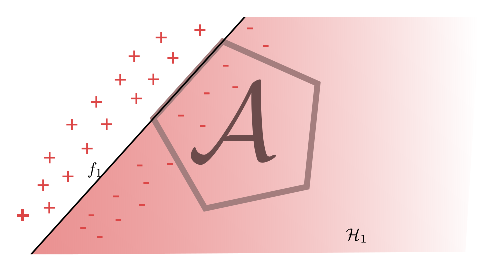
\includegraphics[height=4cm]{object_primitives_2}
			\end{figure}

			\begin{equation}
				\halfspaceprimitive_{\indexi} =
					\left\{
						(\xcoord,\ycoord,\zcoord) \in \world |
						\function_{\indexi}(\xcoord,\ycoord,\zcoord) \leq 0
					\right\}
			\end{equation}

		\end{frame}

		\begin{frame}
			\frametitle{Representation of Bodies}

			A convex polyhedron is then a collection of half-space primitives.

			\begin{figure}[h]
				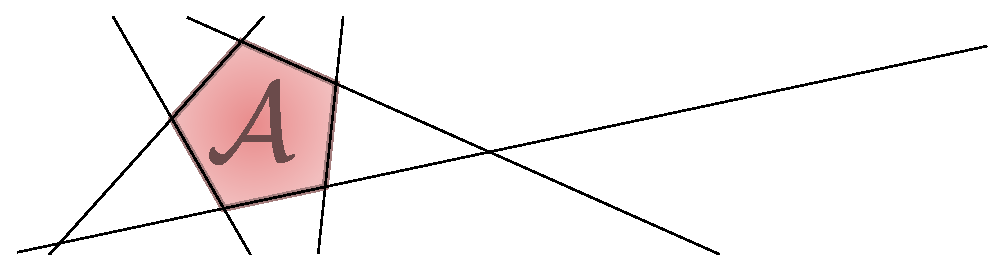
\includegraphics[height=4cm]{object_primitives_3}
			\end{figure}

			\begin{equation}
				\robot =
					\halfspaceprimitive_1 \cap \halfspaceprimitive_2 \cap \cdots \cap
					\halfspaceprimitive_{\cardinality{\robot}}
					\label{eq:convex_robot}
			\end{equation}

		\end{frame}

		\begin{frame}

			\frametitle{Representation of Bodies}

			Complex robot shapes may be built up of a set of convex polyhedra.

			\begin{figure}[h]
				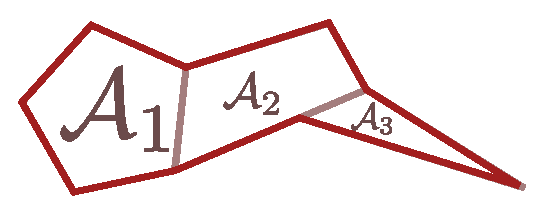
\includegraphics[height=4cm]{object_primitives_4}
			\end{figure}

			\begin{equation}
				\robot =
					\robot_1 \cup \robot_2 \cup \cdots \cup \robot_{\cardinality{\robot}}
					\label{eq:non_convex_robot}
			\end{equation}

		\end{frame}

	\begin{frame}
		\frametitle{Point Collision Detection}

		A point $\point$ may be tested for collision by defining:

		\begin{equation}
			\logicalpredicate_{\indexi} =
				\begin{cases}
					\true, & f_{\indexi} \leq 0 \\
					\false, & f_{\indexi} > 0
				\end{cases}
		\end{equation}

		\begin{figure}[h]
			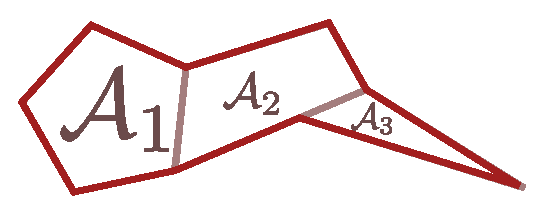
\includegraphics[height=4cm]{object_primitives_4}
		\end{figure}

		\begin{equation}
			\logicalpredicate(\point) =
				\bigvee_{\robot_{\indexi} \in \robot}
					\left(
						\bigwedge_{\halfspaceprimitive_{\indexj} \in \robot_{\indexi}}
							\logicalpredicate_{\indexj}
					\right)
			=
			\begin{cases}
				\true,  &\point \in\robot \\
				\false, &\point \not\in \robot
			\end{cases}
		\end{equation}

	\end{frame}

	\begin{frame}
		\frametitle{Hierarchical Collision Detection}

		\begin{figure}[htb]
			\centering
			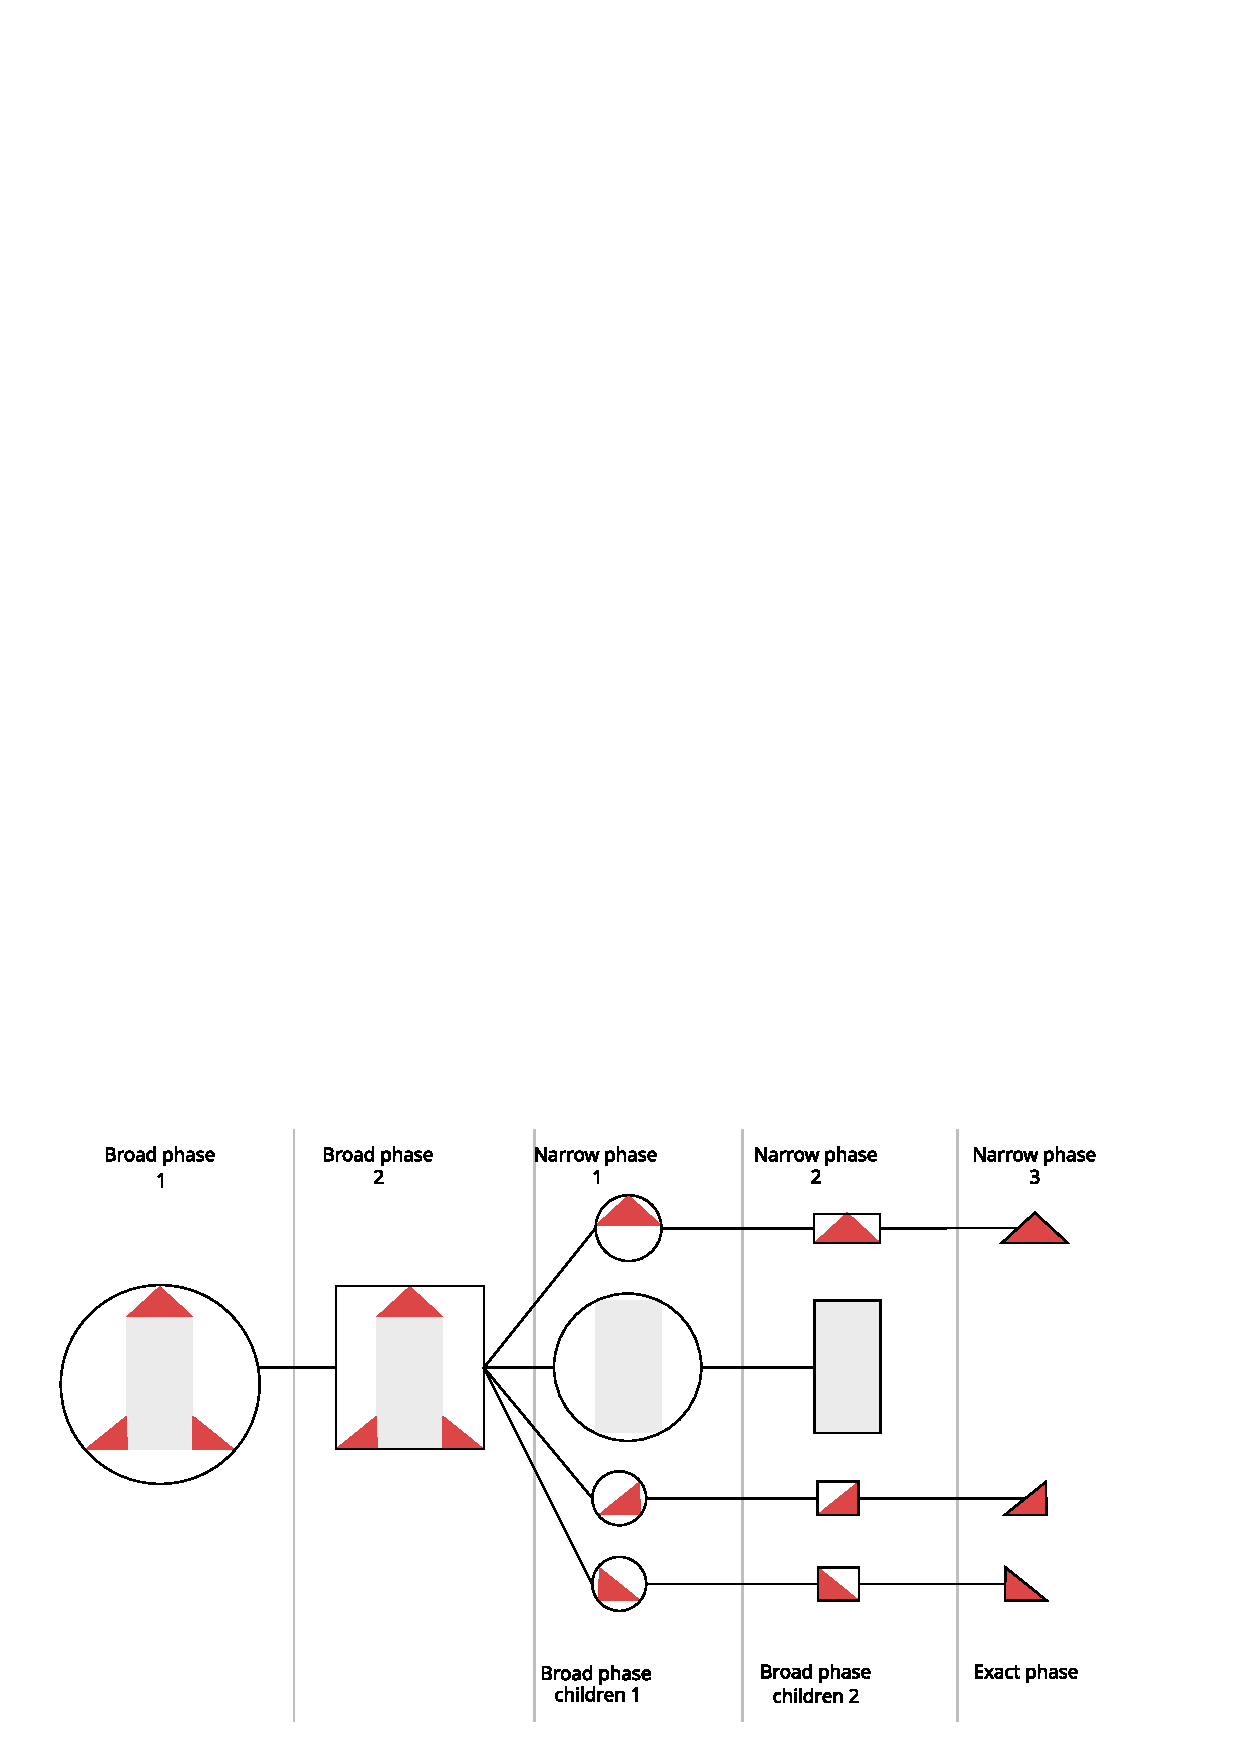
\includegraphics[width=\textwidth]{hierarchical_collision_detection.png}
		\end{figure}
	\end{frame}

	\begin{frame}
		\frametitle{Path Segment Collision Detection}

		Sample points along path, test for collisions.

		\begin{figure}
			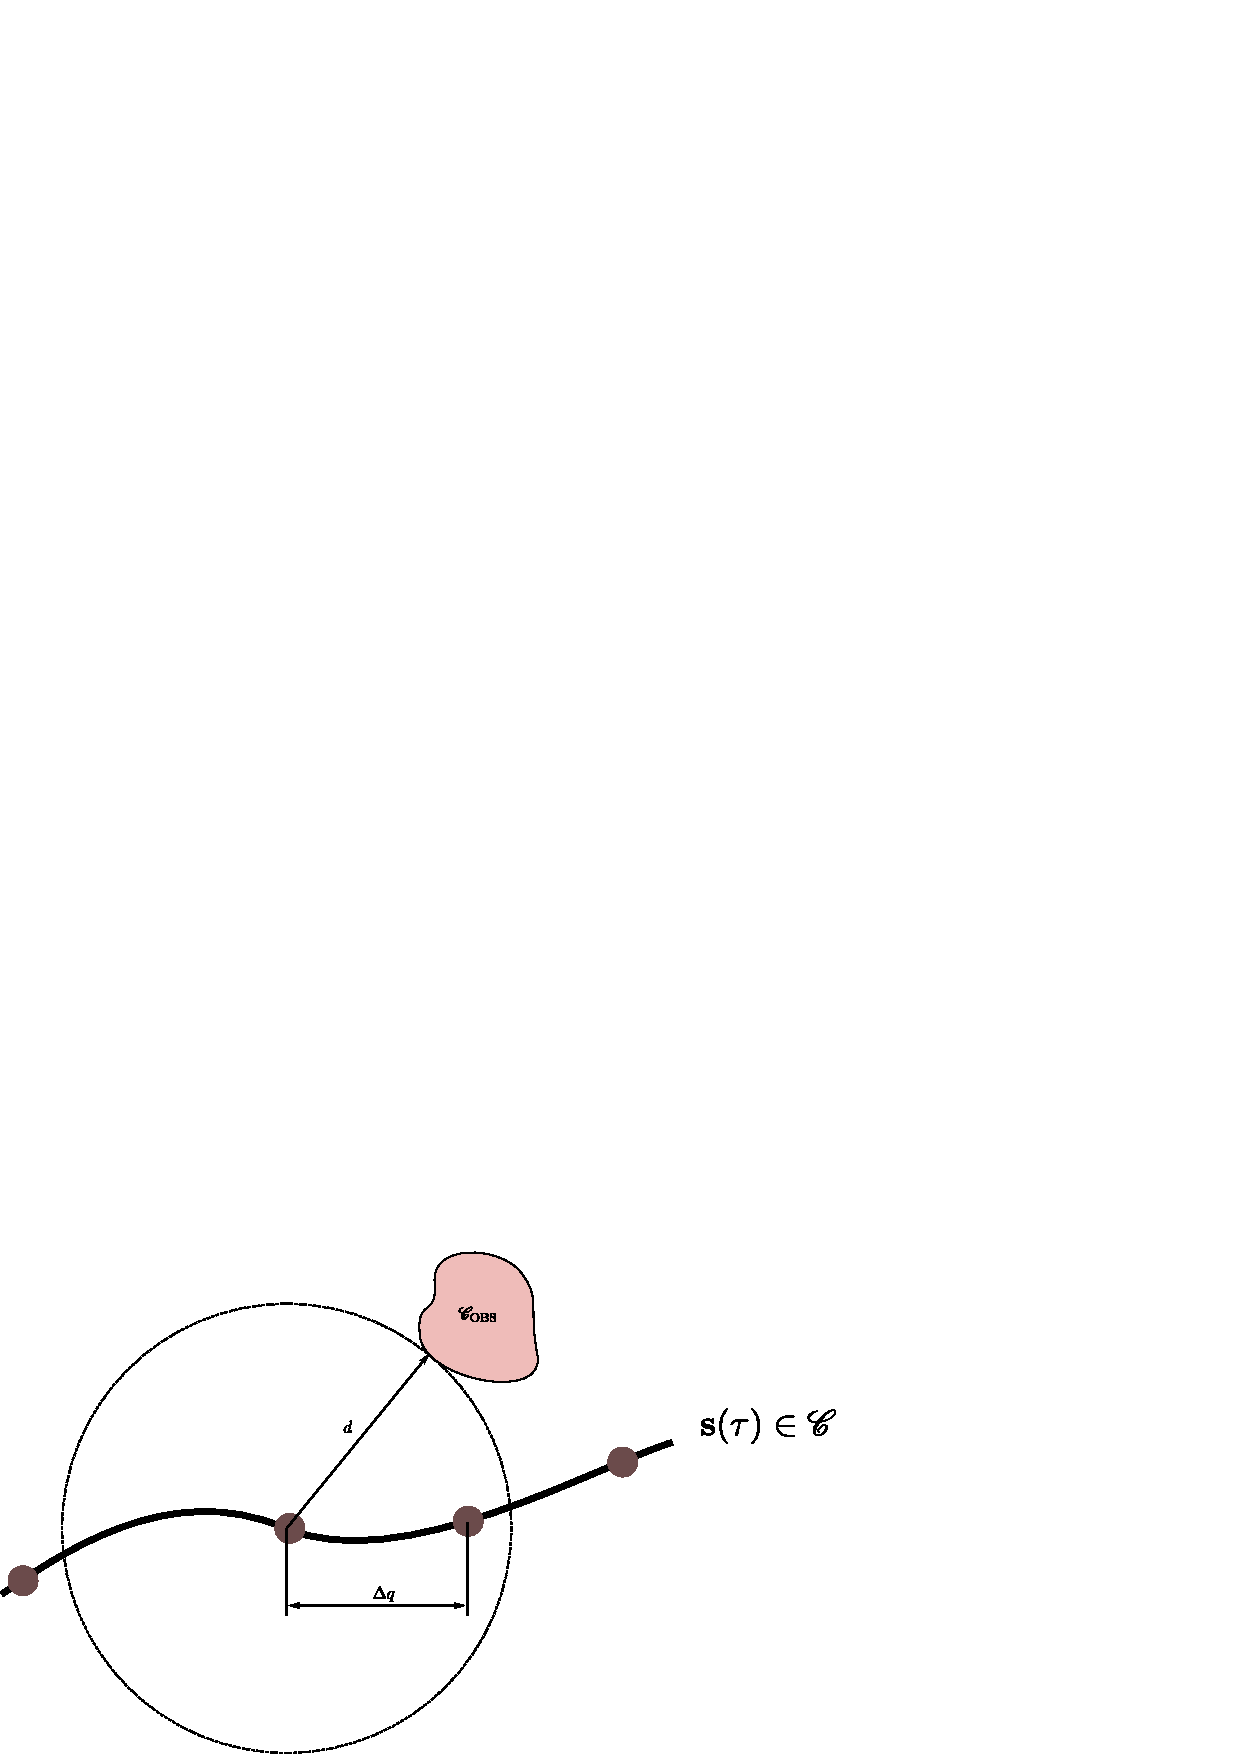
\includegraphics[width=0.8\textwidth]{path_collision_detection.png}
		\end{figure}

		\begin{itemize}

			\item

				Points spaced $\Delta \configuration$ apart

			\item

				$\Delta\configuration$ determined experimentally, or from
				minimum distance to nearest obstacle from collision detection
				algorithms.

		\end{itemize}
	\end{frame}

	\begin{frame}
		\frametitle{Sampling Configuration Space}
		\begin{figure}
			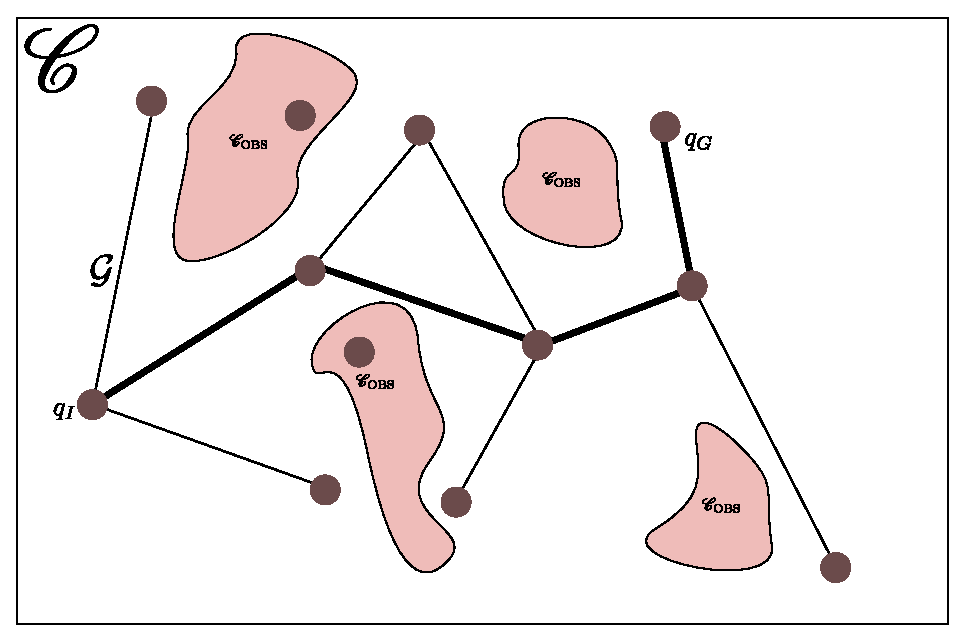
\includegraphics[width=0.8\textwidth]{sampling_methods}
		\end{figure}

		\begin{itemize}
			\item

				Sample Configuration Space

			\item

				Connect samples to obtain topological graph $\topologicalgraph$.

			\item

				Use graph search techniques to find path
		\end{itemize}
	\end{frame}

	\begin{frame}
		\frametitle{Random Trees}

		\begin{itemize}

			\item

				Resolution increases as time increases

			\item

				Can be used under differential constraints

		\end{itemize}

		\begin{figure}[h]
			\centering
			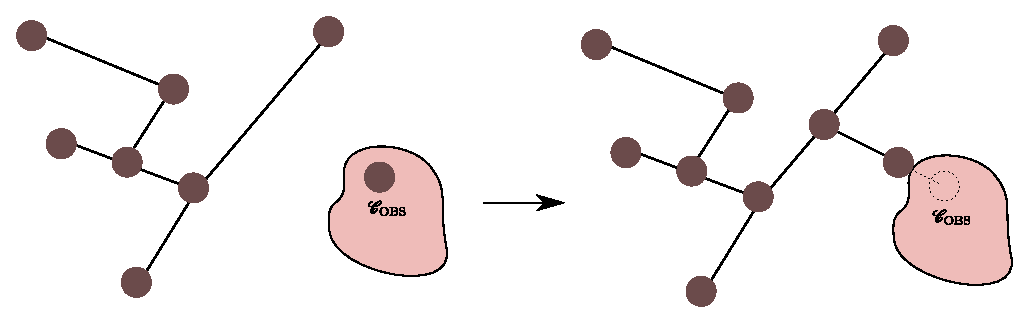
\includegraphics[width=0.7\textwidth]{RRT}
		\end{figure}

		\begin{figure}[h]
			\centering
			\includegraphics[width=0.5\textwidth]{RRT_denseness}
			\caption{[Planning Algorithms, S.M. LaValle]}
		\end{figure}

	\end{frame}

	\begin{frame}
		\frametitle{Smoothing Random Paths}

		\begin{enumerate}

			\item

				Choose two points on the path

			\item

				Merge them smoothly

			\item

				Test new path for collisions
		\end{enumerate}

		\begin{equation}
			\pathsym'(\timenorm) =
				\begin{cases}
					\pathsym(\timenorm) & \timenorm\in[0, \timenorm_1]\\
					%
					\relweight\pathsym(\timenorm_1) +
						(1-\relweight)\pathsym(\timenorm_2)
					& \timenorm\in(\timenorm_1,\timenorm_2)\\
					%
					\pathsym(\timenorm) & \timenorm\in[\timenorm_2, 1]\\
				\end{cases}
		\end{equation}

		\begin{figure}[h]
			\centering
			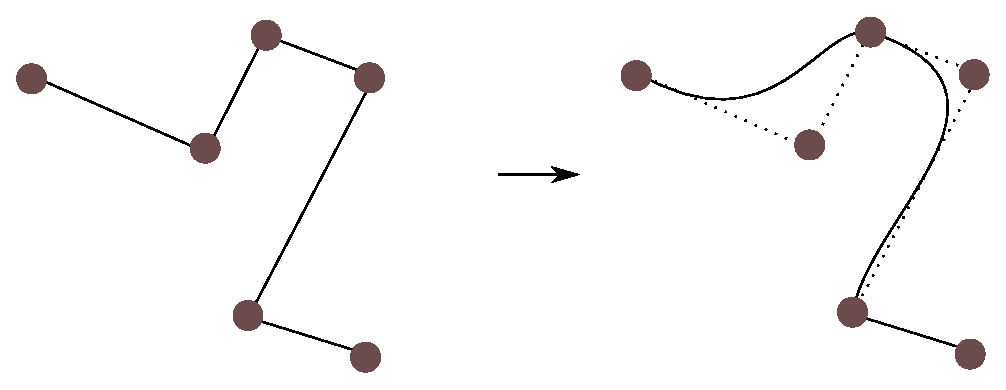
\includegraphics[width=0.8\textwidth]{smoothing_random_paths}
		\end{figure}

	\end{frame}

% ==============================================================================
% Trajectory Generation
% ==============================================================================

\section{Trajectory Generation}

	\begin{frame}
		\frametitle{Overview of Trajectory Generation}

		\begin{itemize}

			\item

				Path $\pathsym(\timenorm)$ has been found

			\item

				Find trajectory $\timenorm = \function(\timesym)$ along this
				path
		\end{itemize}

		\begin{figure}[hb]
			\centering
			\def\svgwidth{\columnwidth}
			\import{res/img/}{trajectory_generation_categories.pdf_tex}
		\end{figure}
	\end{frame}

	\begin{frame}
		\frametitle{Elementary Trajectories}

		\begin{itemize}

			\item

				Polynomial

				\begin{itemize}

				%	\item

				%		Most basic

					\item

						Higher derivatives become zero

				\end{itemize}

				\begin{equation}
					\timenorm(\timesym)
						= \polynomial
						= \sum_{\indexi=0}^{\poldeg}
						\coefficient_{\indexi} \timesym^{\indexi}
				\end{equation}

			\item

				Trigonometric

				\begin{itemize}

					\item

						Good for continuous cyclic motions

					\item

						Of type $\contdeg{\infty}$
				\end{itemize}

				\begin{equation}
					\timenorm(\timesym) =
						\frac{%
								\timenorm_{\final} - \timenorm_0
							}
							{%
								2
							}
						\left(
							1 - \cos
								\frac{%
										\pi(\timesym - \timesym_0)
									}
									{%
										\timesym_{\final} - \timesym_0
									}
						\right)
						+ \timenorm_0
				\end{equation}

			\item

				Exponential

				\begin{itemize}

					\item

						Exponential in velocity profile

					\item

						Degree of continuity may be chosen by setting parameters
				\end{itemize}

				\begin{equation}
					\timenorm(\timesym) = \gain_1\int_{0}^{\timesym}
						e^{-\gain_2 f(\timesym, \gain_3)} \der \timesym
				\end{equation}

		\end{itemize}
	\end{frame}

	\begin{frame}
		\frametitle{Trajectory Composition}

		Elementary trajectories may be combined with bends.

		\begin{itemize}

			\item

				Circular bends

			\item

				Polynomial bends

				Forms the basis of spline interpolation techniques

			\item

				Trigonometric bends

		\end{itemize}

		\begin{figure}
			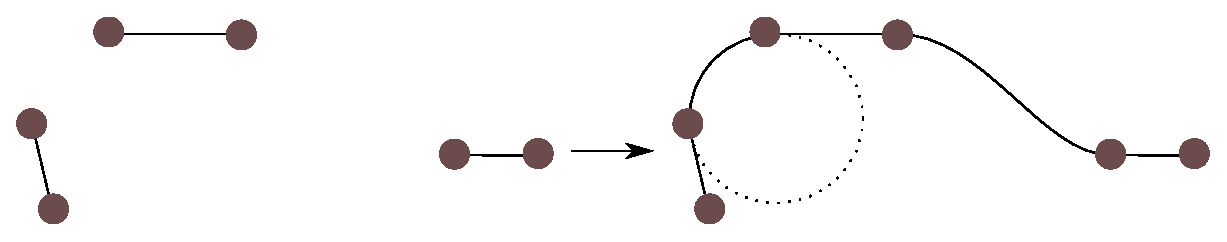
\includegraphics[width=\textwidth]{trajectory_composition}
		\end{figure}

		Type of bend determines level of continuity at transitions

	\end{frame}

	\begin{frame}
		\frametitle{Approximation Techniques}

		Smoothing Splines

		\begin{itemize}
			\item

				Find a polynomial $\polynomial$ that balances the error in
				approximation to the total curvature

			\item

				Do binary search over $\relweight$ to guarantee maximum error
		\end{itemize}

		\begin{equation}
			\argmin_{\polynomial}
			\left\{
				\relweight
				\underbrace{%
					\sum_{\indexi = 0}^{\cardinality{\setofpoints}}
						\gain_{\indexi}
						{%
							\left(
								\polynomial(\timesym_{\indexi}) -
								\point_{\indexi}
							\right)
						}^2
				}_{\text{error in approximation}}
				+
				(1 - \relweight)
				\underbrace{%
					\int_{\timesym_0}^{\timesym_{\cardinality{\setofpoints}}}
						\ddot{\polynomial}^2
					\der \timesym
				}_{\text{curvature}}
			\right\}
			\label{eq:smoothing_cubic_splines_criterion}
		\end{equation}
	\end{frame}

	\begin{frame}
		\frametitle{Approximation Techniques}

		Polynomial bends

		\begin{itemize}
			\item

				Simple for straigh-line trajectories

			\item

				Easy to guarantee an accuracy tolerance $\tol$
		\end{itemize}

		\begin{figure}[hb]
			\centering
			\def\svgwidth{\columnwidth}
			\import{res/img/}{linear_interpolation_with_polynomial_bends.pdf_tex}
		\end{figure}
	\end{frame}

	\begin{frame}
		\frametitle{Trajectory Scaling}

		By changing the duration of the trajectory in certain sections of the
		path, one can avoid exceeding kinematic constraints.


		Make a substitution:

		\begin{equation}
			\timesym = \gain\timesym'
			\label{eq:linear_time_scaling}
		\end{equation}

		This effects the derivatives:

		\begin{equation}
			\tdern{\configuration'}{\indexi}(\timesym') = \gain^{\indexi}
				\tdern{\configuration}{\indexi}(\timesym)
		\end{equation}

		$\gain$ has a direct impact on the maximum value of
		$\configuration(\timesym)$.

		\begin{equation}
			\gain = \min
				\left\{
					\sqrt[\indexi]
					{%
						\frac
						{%
							\constraint_{\indexi}
						}
						{%
								\norm
								{%
									\tdern{\configuration}{\indexi}(\timesym)
								}_{\max}
						}
					}
					\quad
					\forall \constraint_{\indexi} \in \setofconstraints
				\right\}
		\end{equation}


	\end{frame}
% ==============================================================================
% CDPR Modelling
% ==============================================================================

\section{CDPR Modelling}

	\begin{frame}
		\frametitle{CDPR Geometric Model}
        \begin{figure}[hb]
			\centering
			\def\svgwidth{\columnwidth}
			\import{res/img/}{geometry_of_cdpr.pdf_tex}
        \end{figure}

		Loop Closure:

		\begin{equation}
			\project{%
				\proximalanchor_{\indexi}
			}{\world}
			- \transvec
			- \rotmat{\world}{\platform}
				\project{%
					\distalanchor_{\indexi}
				}{\platform}
			- \cablevec_{\indexi}
			=
			\zerovec
			\label{eq:cdpr_loop_closure}
		\end{equation}

	\end{frame}

	\begin{frame}
		\frametitle{CDPR Geometric Model}
        \begin{figure}[hb]
			\centering
			\def\svgwidth{\columnwidth}
			\import{res/img/}{geometry_of_cdpr.pdf_tex}
        \end{figure}

		Leads directly to inverse geometric model:

		\begin{equation}
			\cablelengths
				= \left[
					\begin{matrix}
						\norm{\cablevec_1} \\
						\vdots \\
						\norm{\cablevec_{\numcables}}
					\end{matrix}
				\right]
				= \invgeometricmodel(\pose)
				= \left[
					\begin{matrix}
						\norm
						{%
							\project{\proximalanchor_1}{\world}
							- \transvec
							- \rotmat{\world}{\platform}\project{\distalanchor_1}{\platform}
						}
						\\
						\vdots
						\\
						\norm
						{%
							\project{\proximalanchor_{\numcables}}{\world}
							- \transvec
							- \rotmat{\world}{\platform}\project{\distalanchor_{\numcables}}{\platform}
						}
					\end{matrix}
				\right]
			\label{eq:cdpr_inverse_geometric_model}
		\end{equation}

	\end{frame}

	\begin{frame}
		\frametitle{Inverse Kinematic Model}

        \begin{figure}[hb]
			\centering
			\def\svgwidth{\columnwidth}
			\import{res/img/}{geometry_of_cdpr.pdf_tex}
        \end{figure}

		Found through derivation of the inverse geometric model:

        \begin{equation}
            \dot{\cablelengths}
                =   \invkinematicmodel(\pose, \dot{\pose})
                =   \frac
                    {%
                        \partial\invgeometricmodel(\pose)
                    }
                    {%
                        \partial\timesym
                    }
                =   \frac
                    {%
                        \partial\invgeometricmodel(\pose)
                    }
                    {%
                        \partial\pose
                    }
                    \frac
                    {%
                        \partial\pose
                    }
                    {%
                        \partial\timesym
                    }
                =   \invgeometricjac\dot{\pose}
        \end{equation}
	\end{frame}

	\begin{frame}
		\frametitle{Wrench Closure}
		\begin{figure}[hb]
			\centering
			\def\svgwidth{\columnwidth}
			\import{res/img/}{geometry_of_cdpr.pdf_tex}
		\end{figure}

		For Equilibrium:

        \begin{align}
            \sum_{\indexi = 1}^{\numcables}
                \force_{\indexi} +
            \force_{\platform} &= \zerovec \\
            %
            \sum_{\indexi = 1}^{\numcables}
                \distalanchor_{\indexi} \times \force_{\indexi} +
            \torque_{\platform} &= \zerovec
        \end{align}
	\end{frame}

	\begin{frame}
		\frametitle{Wrench Closure}
		\begin{figure}[hb]
			\centering
			\def\svgwidth{\columnwidth}
			\import{res/img/}{geometry_of_cdpr.pdf_tex}
		\end{figure}

		In matrix form:

        \begin{equation}
            \strucmat(\transvec, \rotmatbare)\forcemagvec +
            \wrench_{\platform} = \zerovec
            \label{eq:structure_equation}
        \end{equation}

	\end{frame}

	\begin{frame}

		Equilibrium:

        \begin{align}
            \sum_{\indexi = 1}^{\numcables}
                \force_{\indexi} +
            \force_{\platform} &= \zerovec \\
            %
            \sum_{\indexi = 1}^{\numcables}
                \distalanchor_{\indexi} \times \force_{\indexi} +
            \torque_{\platform} &= \zerovec
        \end{align}

		Matrix form:

        \begin{equation}
            \strucmat(\transvec, \rotmatbare)\forcemagvec +
            \wrench_{\platform} = \zerovec
            \label{eq:structure_equation}
        \end{equation}

		Some poses cannot be supported by the platform.

		Cables need to be in tension

		Wrench-Closure condition:

		\begin{equation}
			\forall
				\left(
					{\wrench}_{\platform}\in\Re^{\robotdof}
				\right)
			\exists
				\left(
					\forcemagvec\in\Re^{\numcables}
				\right)
			\quad\suchthat\quad
				\left(
					\strucmat(\transvec, \rotmatbare)\forcemagvec + \wrench_{\platform} = \zerovec
				\right)
				\wedge
				\left(
					\forcemagvec > \zerovec
				\right)
			\label{eq:wrench_closure_constraint}
		\end{equation}

	\end{frame}

	\begin{frame}
		\frametitle{Workspace of CDPR}

		\begin{columns}
			\column{0.5\textwidth}
			Criteria on poses in the workspace:

			\begin{itemize}
				\item

					In Wrench-Closure

				\item

					Not in singular configuration

				\item

					Not in self-collision

				\item

					Does not exceed maximum cable lengths

				\item

					\ldots
			\end{itemize}

			\column{0.5\textwidth}

			Main approaches:

			\begin{itemize}

				\item

					Discrete samples

					\begin{itemize}
						\item

							Easy to compute

						\item

							Makes no guarantee on points between samples
					\end{itemize}

				\item

					Interval Analysis

					\begin{itemize}

						\item

							Expensive to compute

						\item

							Perfectly guarantees points within interval bounds

					\end{itemize}
			\end{itemize}
		\end{columns}
	\end{frame}


% ==============================================================================
% Conclusion
% ==============================================================================

	\begin{frame}
		\frametitle{Proposed Architecture}
		\begin{figure}[hb]
			\footnotesize
			\centering
			\def\svgwidth{\columnwidth}
			\import{res/img/}{proposed_architecture.pdf_tex}
		\end{figure}
	\end{frame}



\end{document}
